\documentclass{beamer}

\mode<presentation> {

%\usetheme{default}
%\usetheme{AnnArbor}
%\usetheme{Antibes}
%\usetheme{Bergen}
%\usetheme{Berkeley}
%\usetheme{Berlin}
%\usetheme{Boadilla}
%\usetheme{CambridgeUS}
%\usetheme{Copenhagen}
%\usetheme{Darmstadt}
%\usetheme{Dresden}
%\usetheme{Frankfurt}
%\usetheme{GoettBen}
%\usetheme{Hannover}
%\usetheme{Ilmenau}
%\usetheme{JuanLesPins}
%\usetheme{Luebeck}
\usetheme{Madrid}
%\usetheme{Malmoe}
%\usetheme{Marburg}
%\usetheme{Montpellier}
%\usetheme{PaloAlto}
%\usetheme{Pittsburgh}
%\usetheme{Rochester}
%\usetheme{SBapore}
%\usetheme{Szeged}
%\usetheme{Warsaw}

%\usecolortheme{albatross}
%\usecolortheme{beaver}
%\usecolortheme{beetle}
%\usecolortheme{crane}
%\usecolortheme{dolphin}
%\usecolortheme{dove}
%\usecolortheme{fly}
\usecolortheme{lily}
%\usecolortheme{orchid}
%\usecolortheme{rose}
%\usecolortheme{seagull}
%\usecolortheme{seahorse}
%\usecolortheme{whale}
%\usecolortheme{wolverine}

%\setbeamertemplate{footline} % To remove the footer line in all slides uncomment this line
%\setbeamertemplate{footline}[page number] % To replace the footer line in all slides with a simple slide count uncomment this line

%\setbeamertemplate{navigation symbols}{} % To remove the navigation symbols from the bottom of all slides uncomment this line
}

\usepackage{graphicx} % Allows includB images
\usepackage{booktabs} % Allows the use of \toprule, \midrule and \bottomrule in tables
\setbeamertemplate{enumerate item}{\insertenumlabel.}
\usepackage{dcolumn}
\usepackage{tcolorbox}
\usepackage{lipsum}
\usepackage{chronology}
\beamertemplatenavigationsymbolsempty

%----------------------------------------------------------------------------------------
%	TITLE PAGE
%----------------------------------------------------------------------------------------

\title[VAM ft. The Replication Project]{\textbf{The \textit{dplyr} Package in R}} % The short title appears at the bottom of every slide, the full title is only on the title page
\subtitle{Write less and faster code}
\author{Selina Hofstetter} % Your name
\institute[LSE] % Your institution as it will appear on the bottom of every slide, may be shorthand to save space
{VAM 1 - MT 2018 \\ % Your institution for the title page
\medskip
%\textit{Please do not circulate}
\medskip
}
\date{October 17, 2018} % Date, can be changed to a custom date

\begin{document}

\begin{frame}
\titlepage % Print the title page as the first slide
\end{frame}

%----------------------------------------------------------------------------------------
%	PRESENTATION SLIDES
%----------------------------------------------------------------------------------------

%------------------------------------------------
\section{Introduction} 
%------------------------------------------------
% (1)
\begin{frame}
\frametitle{The \href{https://www.tidyverse.org}{tidyverse} package}
\begin{columns}
\column{0.45	\textwidth}
\begin{center}
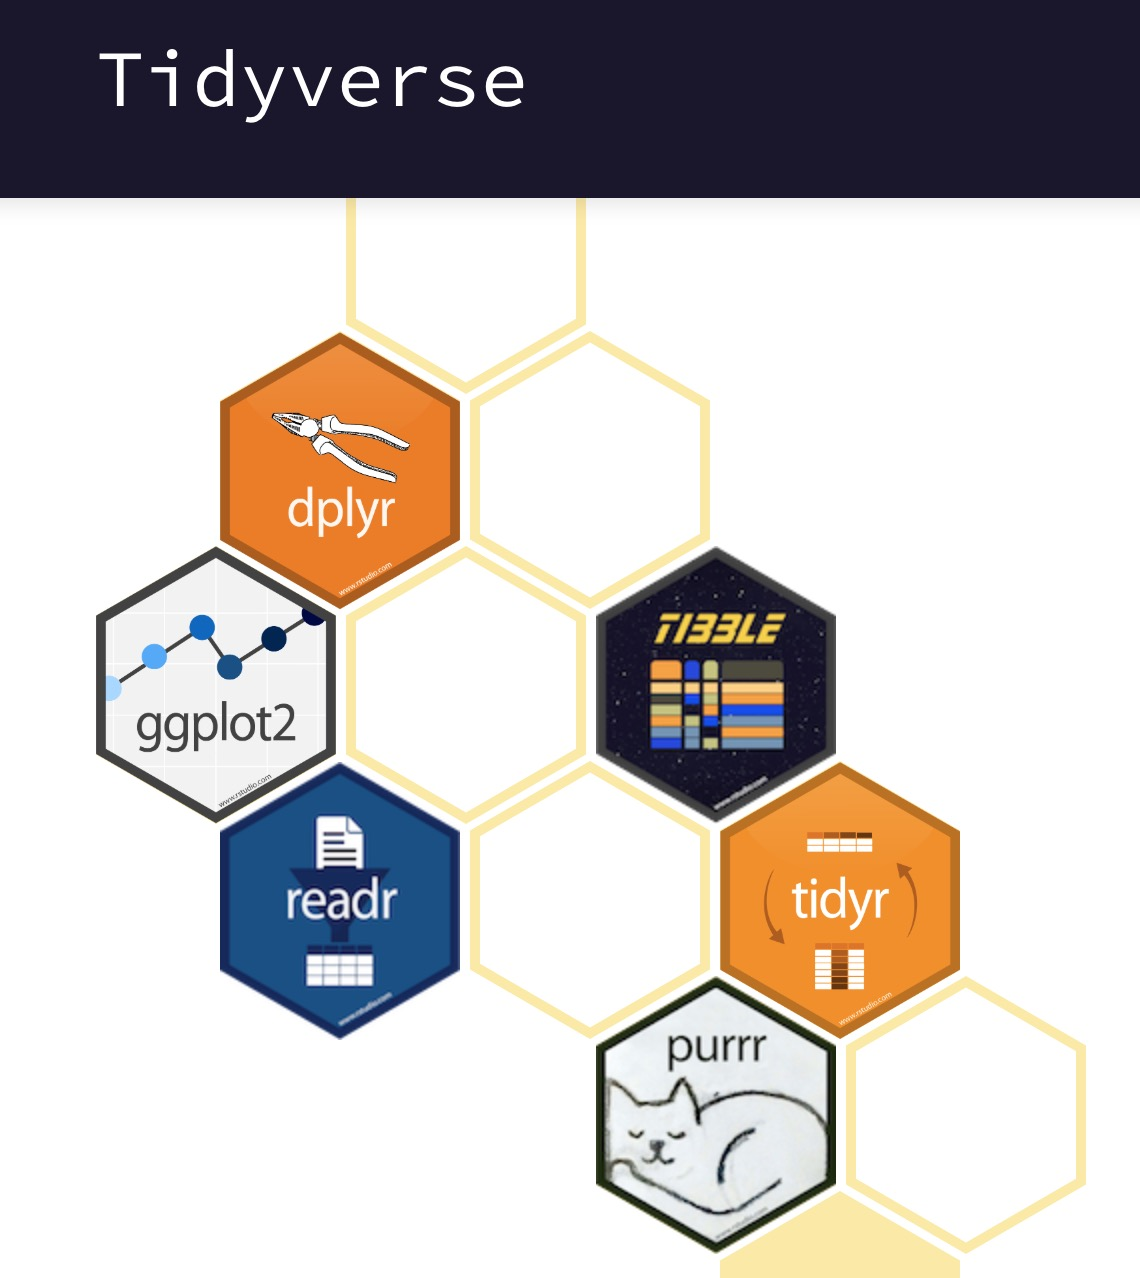
\includegraphics[width=0.9\textwidth]{tidy.jpg}
\end{center}
\column{0.55\textwidth} 
\begin{center}
\begin{itemize}
\item Created by {\color{blue}{\href{http://hadley.nz/}{Hadley Wickham}}}
\end{itemize}
\end{center}
\end{columns}
\end{frame}

% (2)
\begin{frame}
\frametitle{The \href{https://www.tidyverse.org}{tidyverse} package}
\begin{columns}
\column{0.45	\textwidth}
\begin{center}
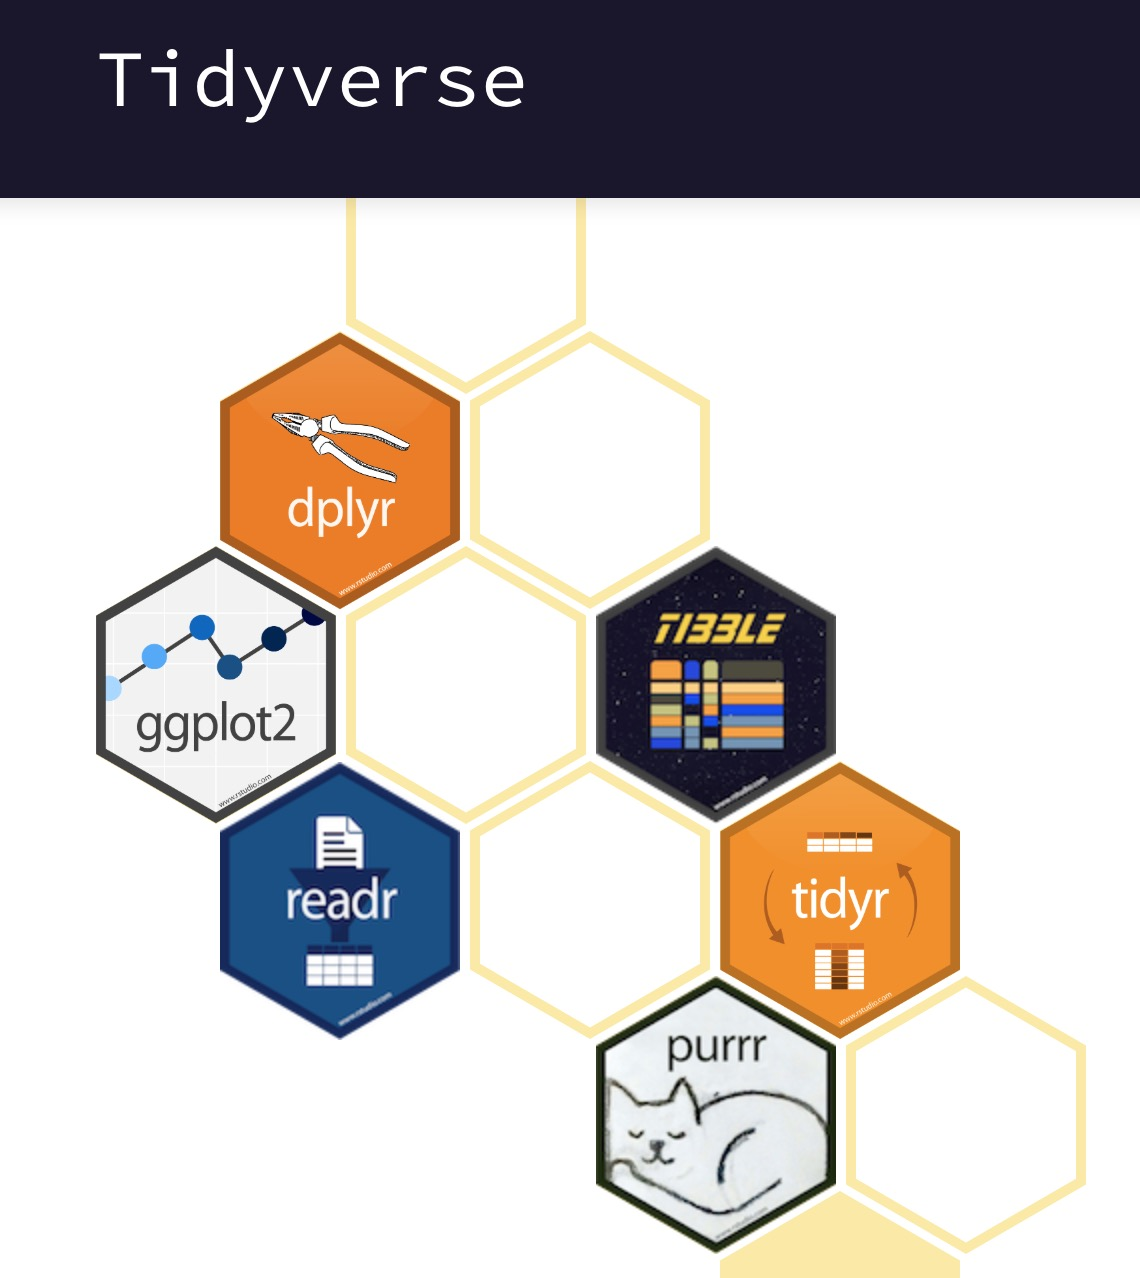
\includegraphics[width=0.9\textwidth]{tidy.jpg}
\end{center}
\column{0.55\textwidth} 
\begin{center}
\begin{itemize}
\item Created by {\color{blue}{\href{http://hadley.nz/}{Hadley Wickham}}}
\item Helps you to organise, manipulate and analyse your data
\end{itemize}
\end{center}
\end{columns}
\end{frame}

% (3)
\begin{frame}
\frametitle{The \href{https://www.tidyverse.org}{tidyverse} package}
\begin{columns}
\column{0.45	\textwidth}
\begin{center}
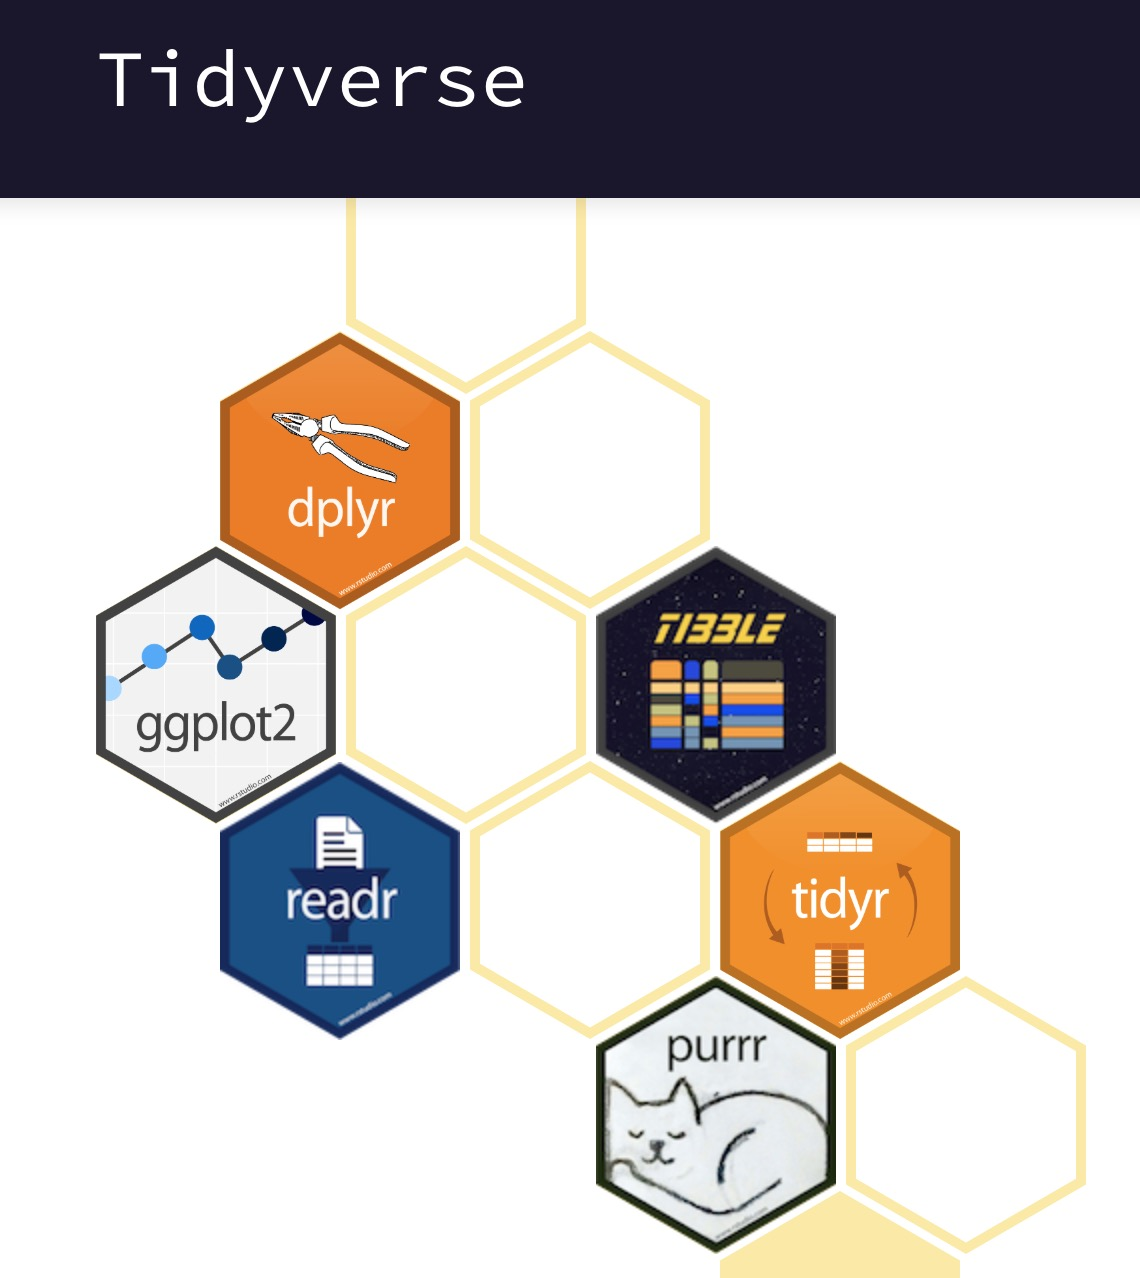
\includegraphics[width=0.9\textwidth]{tidy.jpg}
\end{center}
\column{0.55\textwidth} 
\begin{center}
\begin{itemize}
\item Created by {\color{blue}{\href{http://hadley.nz/}{Hadley Wickham}}}
\item Helps you to organise, manipulate and analyse your data
\item (Probably at most times) faster than your own code 
\end{itemize}
\end{center}
\end{columns}
\end{frame}

% (4)
\begin{frame}
\frametitle{The \href{https://www.tidyverse.org}{tidyverse} package}
\begin{columns}
\column{0.45	\textwidth}
\begin{center}
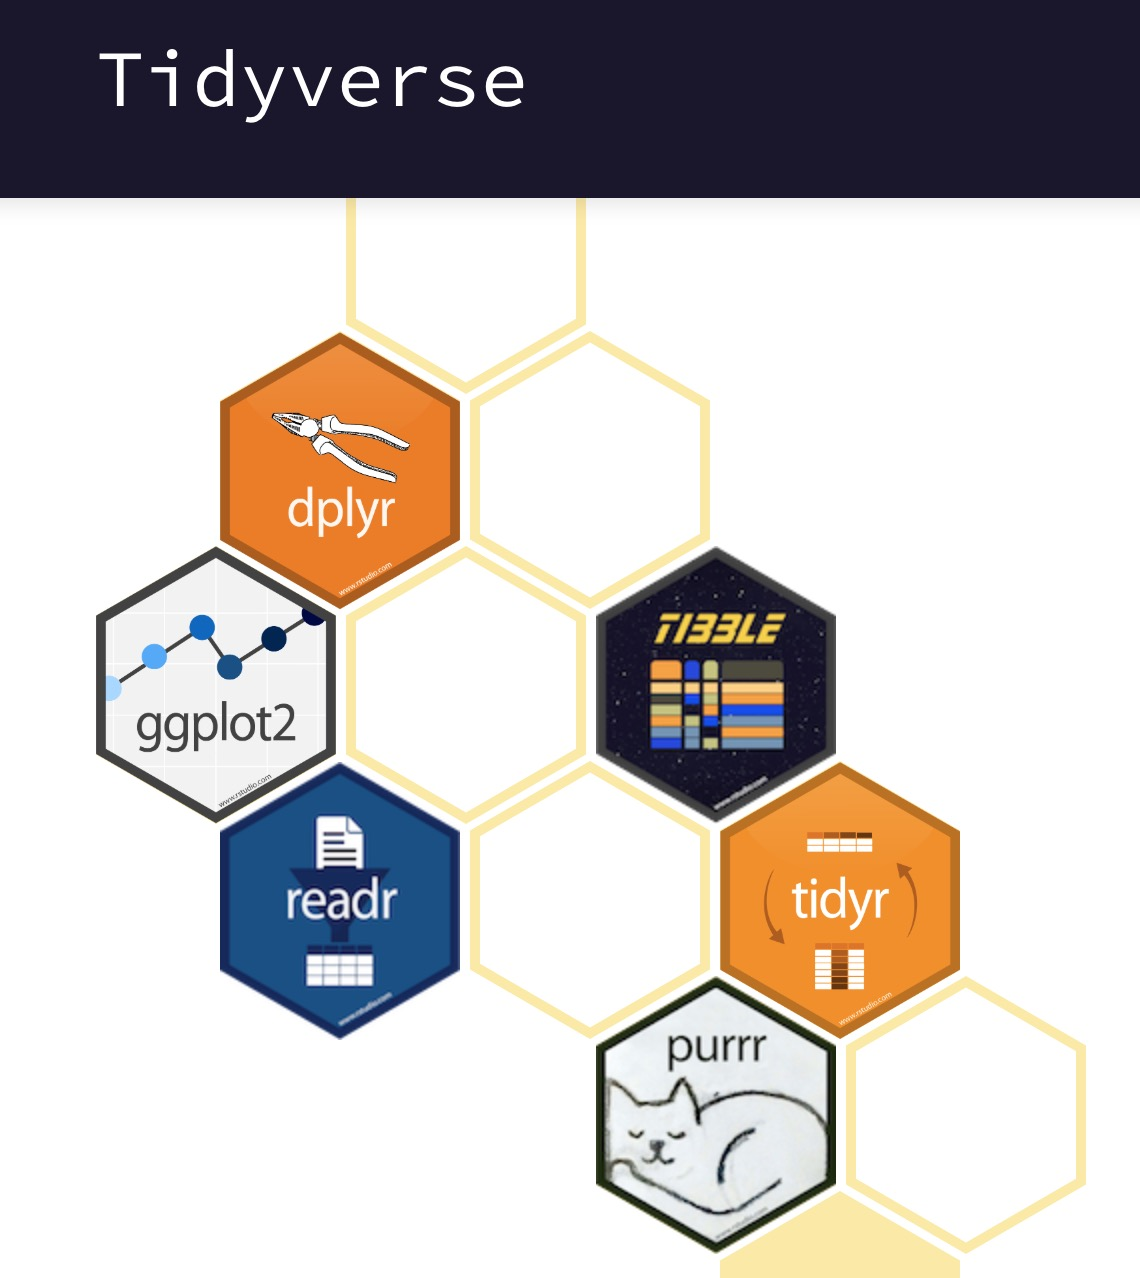
\includegraphics[width=0.9\textwidth]{tidy.jpg}
\end{center}
\column{0.55\textwidth} 
\begin{center}
\begin{itemize}
\item Created by {\color{blue}{\href{http://hadley.nz/}{Hadley Wickham}}}
\item Helps you to organise, manipulate and analyse your data
\item (Probably at most times) faster than your own code 
\item Clean and transparent, easy for others to read your code
\end{itemize}
\end{center}
\end{columns}
\end{frame}

% (5)
\begin{frame}
\frametitle{The \href{https://www.tidyverse.org}{tidyverse} package}
\begin{columns}
\column{0.45	\textwidth}
\begin{center}
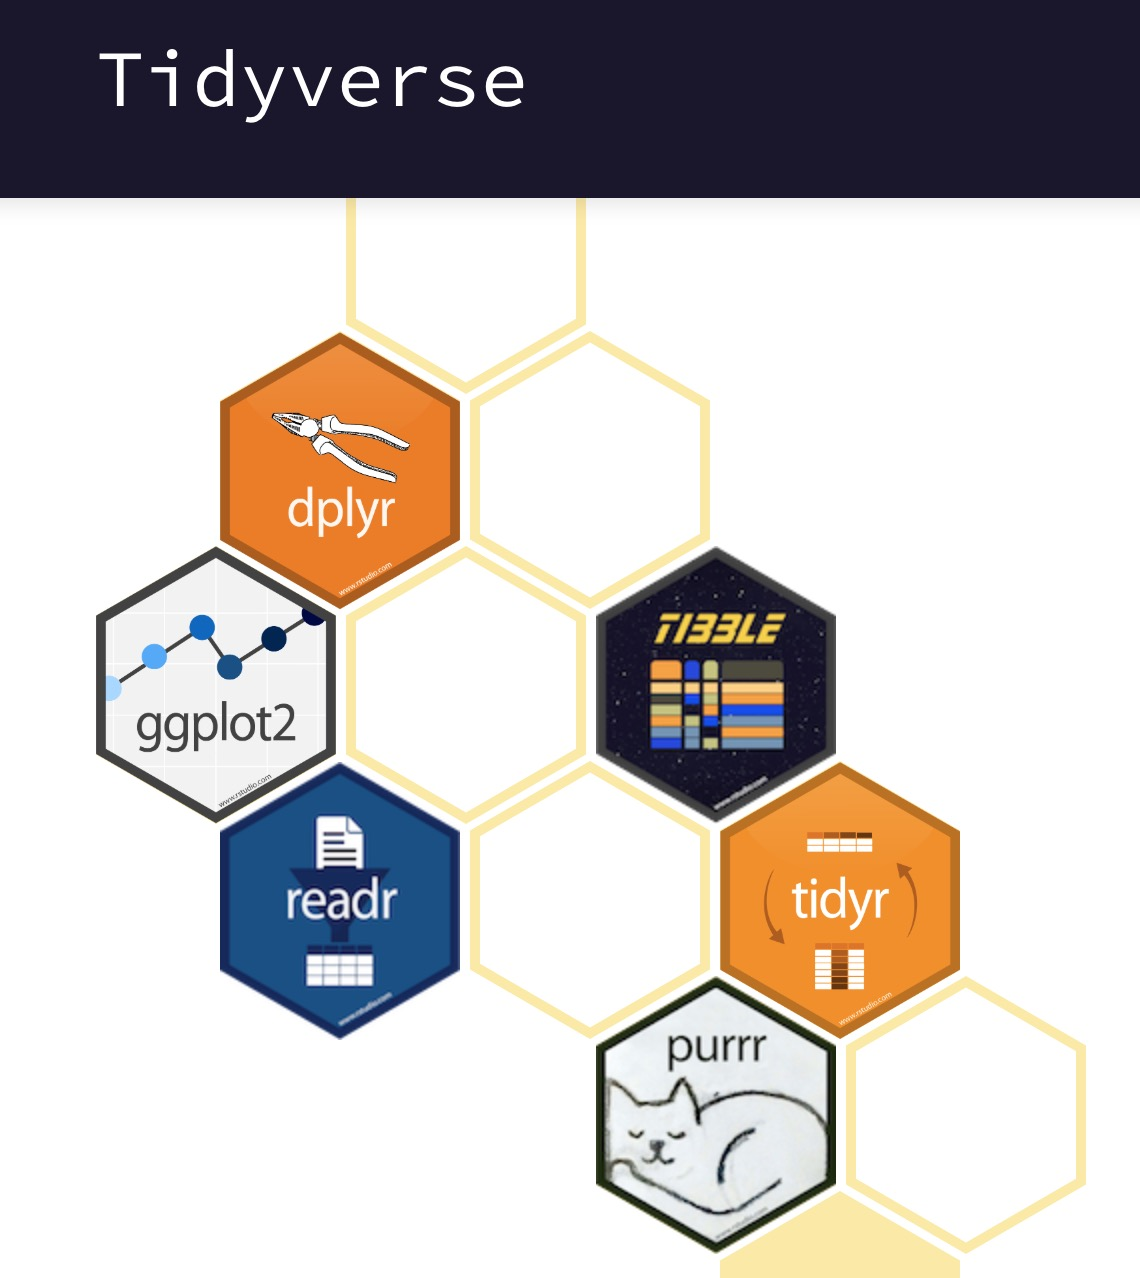
\includegraphics[width=0.9\textwidth]{tidy.jpg}
\end{center}
\column{0.55\textwidth} 
\begin{center}
\begin{itemize}
\item Created by {\color{blue}{\href{http://hadley.nz/}{Hadley Wickham}}}
\item Helps you to organise, manipulate and analyse your data
\item (Probably at most times) faster than your own code 
\item Clean and transparent, easy for others to read your code
\item Requires you to write less
\end{itemize}
\end{center}
\end{columns}
\end{frame}

% (6)
\begin{frame}
\frametitle{The \href{https://www.tidyverse.org}{tidyverse} package}
\begin{columns}
\column{0.45	\textwidth}
\begin{center}
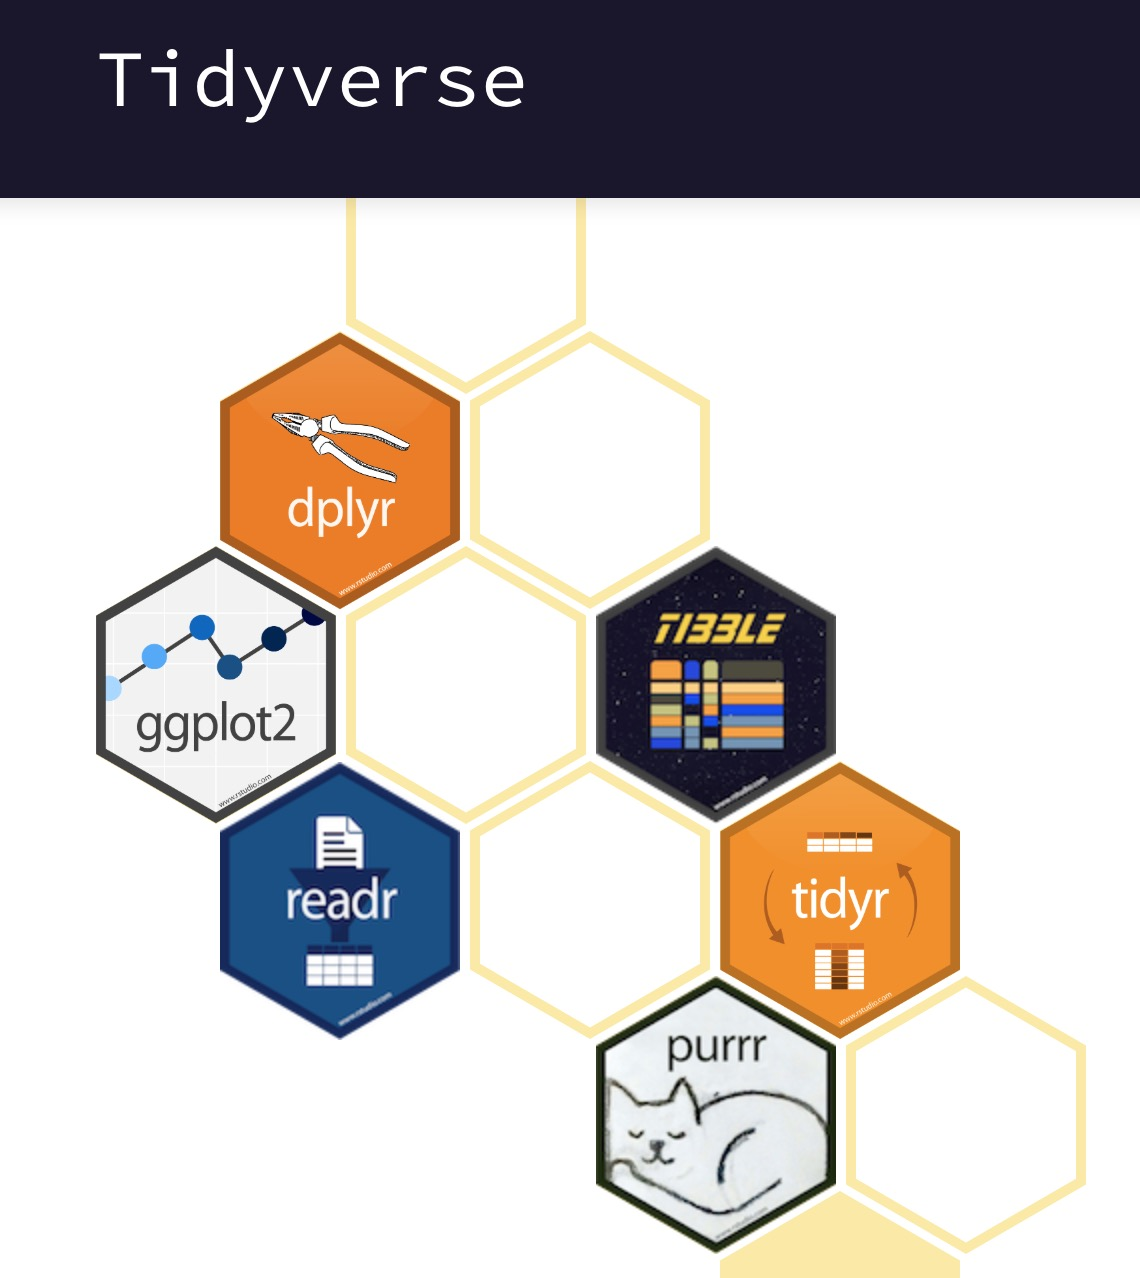
\includegraphics[width=0.9\textwidth]{tidy.jpg}
\end{center}
\column{0.55\textwidth} 
\begin{center}
\begin{itemize}
\item Created by {\color{blue}{\href{http://hadley.nz/}{Hadley Wickham}}}
\item Helps you to organise, manipulate and analyse your data
\item (Probably at most times) faster than your own code 
\item Clean and transparent, easy for others to read your code
\item Requires you to write less
\item My tip: Always think first how you could write code with the help of tidyverse (specifically: dplyr) - avoid long loops!
\end{itemize}
\end{center}
\end{columns}
\end{frame}

%------------------------------------------------
\section{The Verbs}
%------------------------------------------------
% (1)
\begin{frame}
\frametitle{Your \textit{dplyr} toolbox:}
Five verbs to {\color{blue}{manipulate}} your data with:
\begin{itemize}
\item mutate() allows you to generate new variables
\end{itemize}
\begin{center}
{\color{blue}{Example:}}
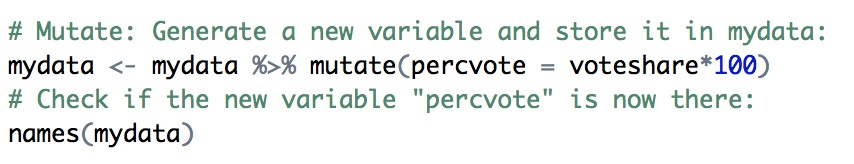
\includegraphics[width=0.9\textwidth]{mutate.jpg}
\end{center}
\end{frame}

% (2)
\begin{frame}
\frametitle{Your \textit{dplyr} toolbox:}
Five verbs to {\color{blue}{manipulate}} your data with:
\begin{itemize}
\item mutate() allows you to generate new variables
\item select() lets you select certain variables in your dataset
\end{itemize}
\begin{center}
{\color{blue}{Example:}}
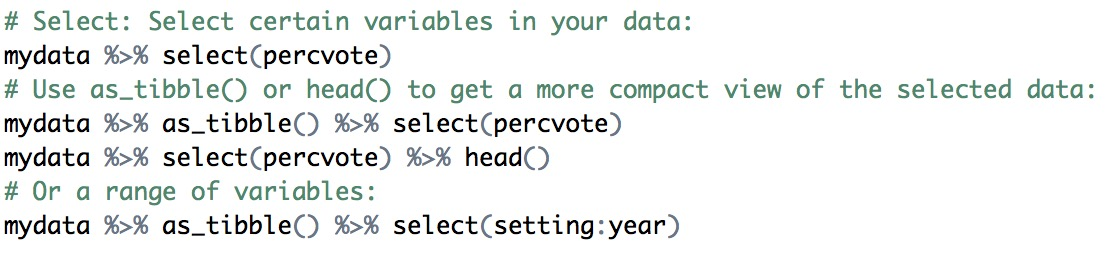
\includegraphics[width=0.9\textwidth]{select.jpg}
\end{center}
\end{frame}

% (3)
\begin{frame}
\frametitle{Your \textit{dplyr} toolbox:}
Five verbs to {\color{blue}{manipulate}} your data with:
\begin{itemize}
\item mutate() allows you to generate new variables
\item select() lets you select certain variables in your dataset
\item filter() enables you to filter out observations of a certain value in your dataset
\end{itemize}
\begin{center}
{\color{blue}{Example:}}
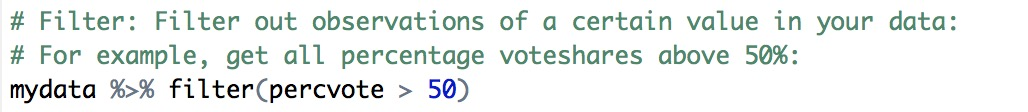
\includegraphics[width=1\textwidth]{filter.jpg}
\end{center}
\end{frame}

% (3)
\begin{frame}
\frametitle{Your \textit{dplyr} toolbox:}
Five verbs to {\color{blue}{manipulate}} your data with:
\begin{itemize}
\item mutate() allows you to generate new variables
\item select() lets you select certain variables in your dataset
\item filter() enables you to filter out observations of a certain value in your dataset
\item summarise() allows you to for example count or calculate the mean value of groups of observations in your data
\end{itemize}
\begin{center}
{\color{blue}{Example:}}
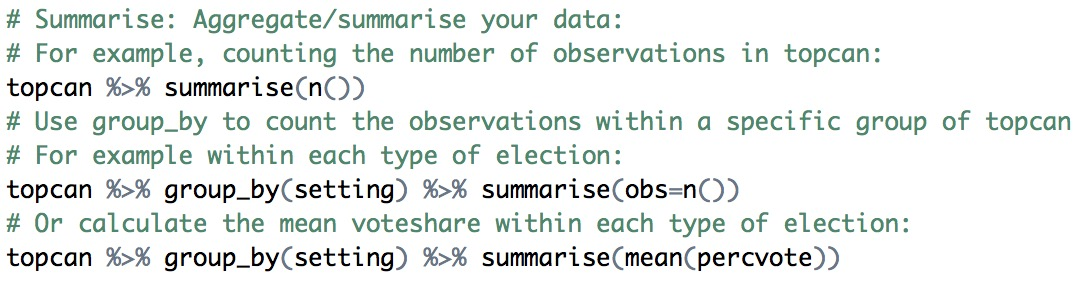
\includegraphics[width=0.9\textwidth]{summarise.jpg}
\end{center}
\end{frame}

% (4)
\begin{frame}
\frametitle{Your \textit{dplyr} toolbox:}
Five verbs to {\color{blue}{manipulate}} your data with:
\begin{itemize}
\item mutate() allows you to generate new variables
\item select() lets you select certain variables in your dataset
\item filter() enables you to filter out observations of a certain value in your dataset
\item summarise() allows you to for example count or calculate the mean value of groups of observations in your data
\item arrange() sorts your data, e.g. alphabetically when you have country-level data
\end{itemize}
\begin{center}
{\color{blue}{Example:}}
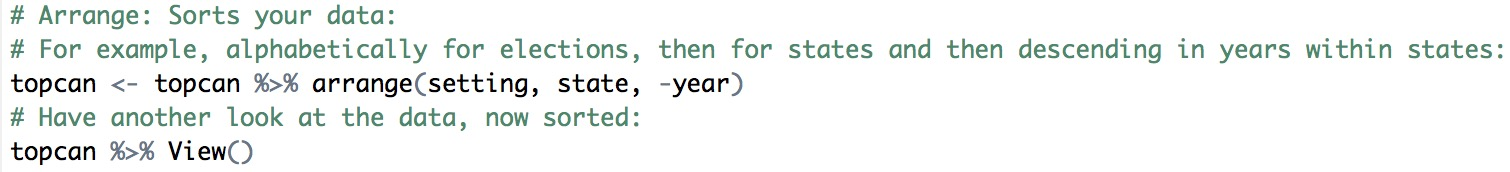
\includegraphics[width=1\textwidth]{arrange.jpg}
\end{center}
\end{frame}



\end{document} 